\section {SERVICE}

\textit{Service} tab is used to configuration parameters of devices which machine contains. Except of set parameters of devices we also set some pressure limits, time limits and devices limit for safe work of machine.\\

IMPORTANT\\
Incorrect setting of the parameters can damage the devices or machine.\\

Tab was divided on several section which each is used to configuration of other device. Sections are:

\begin{itemize}
	\item Power 
	\item MFC
	\item Pump
	\item Vaporaiser
	\item Gases
	\item PID
	\item Time
	\item Motor
\end{itemize}

\subsection{Power}

Section \textit{Power} is used to configuration parameters for power supply. We should specify what is a maximum of power of installed power supply and what is a power limit which user can set. \\\\
Parameters:

\begin{itemize}
	\item \textit{Power limit} - define maximum of power of installed power supply 
	\item \textit{Max power} - define  power limit which user can set
\end{itemize}

	\begin{figure}[!h] 
	\centering 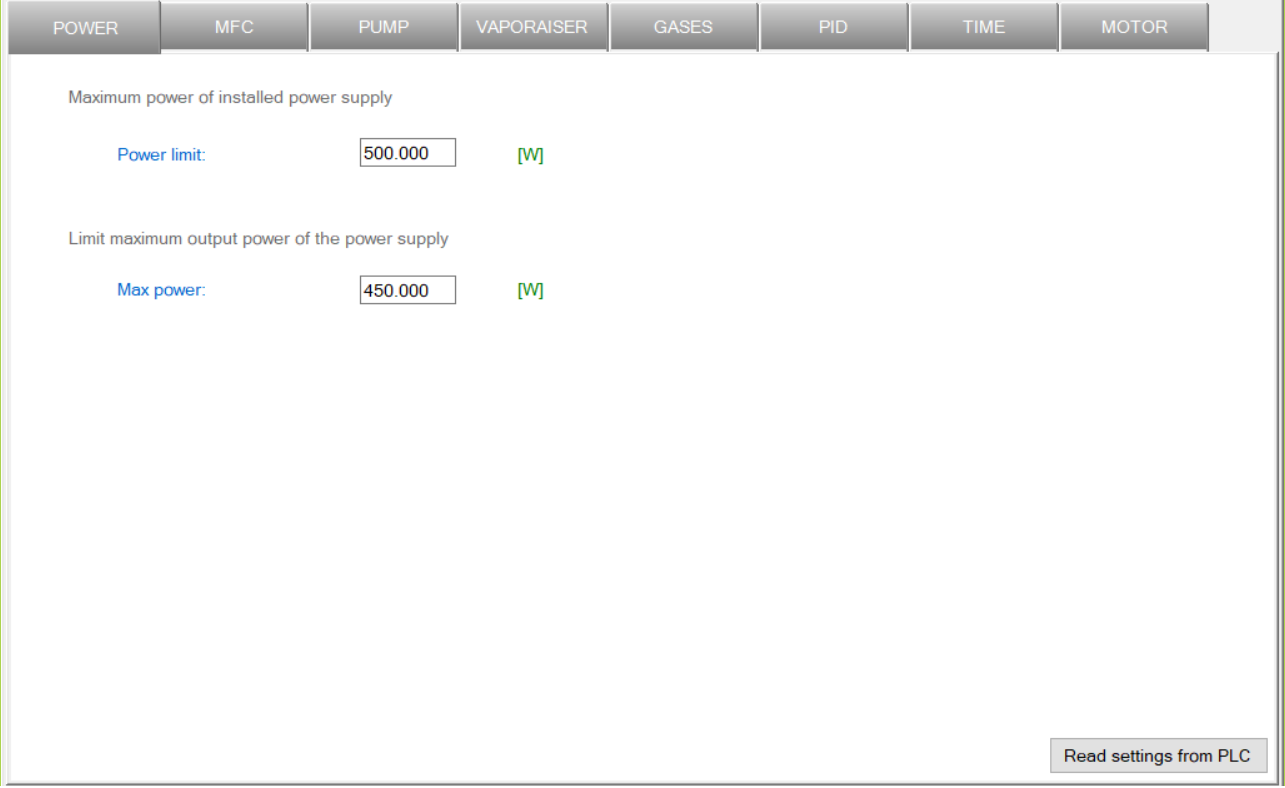
\includegraphics[width=0.8\textwidth]{Graphic/Service/Power.png}	
	\caption{Service - section power}
	\label{alerts_window}
	\end{figure}
	\FloatBarrier

\subsection{MFC}

Section \textit{MFC} is used to configuration parameters for \textit{Mass Flow Controller}. We should define how many controllers are connected to system, for which gas controller has been calibrated, what is a maximum flow and what is a range of voltage to control him. Additionally we specify wait time for stabilization of flow during a process and safety procedure protect of chamber before dangerous mixture of gases.\\\\
Parameters:
\begin{itemize}
	\item \textit{Connection} - determine if corresponding mass flow controller is connected to system
	\item \textit{Calibrated for gas} - specify gas in which has been calibrated mas flow controller
	\item \textit{Maximum gas flow} - determine what is a maximum flow for corresponding mass flow controller
	\item \textit{Voltage} - determine what is a range of voltage used to control of corresponding mass flow controller
	\item \textit{Flow stabilization time} - determine wait time for stabilization of flow. When time passes, system will be check flow is in specific range by process.
	\item \textit{Flow stabilization time of safety mix gas flow meter} - determine wait time for stabilization of flow. When time passes, system will be check flow is in specific range determined by safety procedure used to protect of chamber before dangerous mixture of gases.
\end{itemize}

	\begin{figure}[!h] 
	\centering 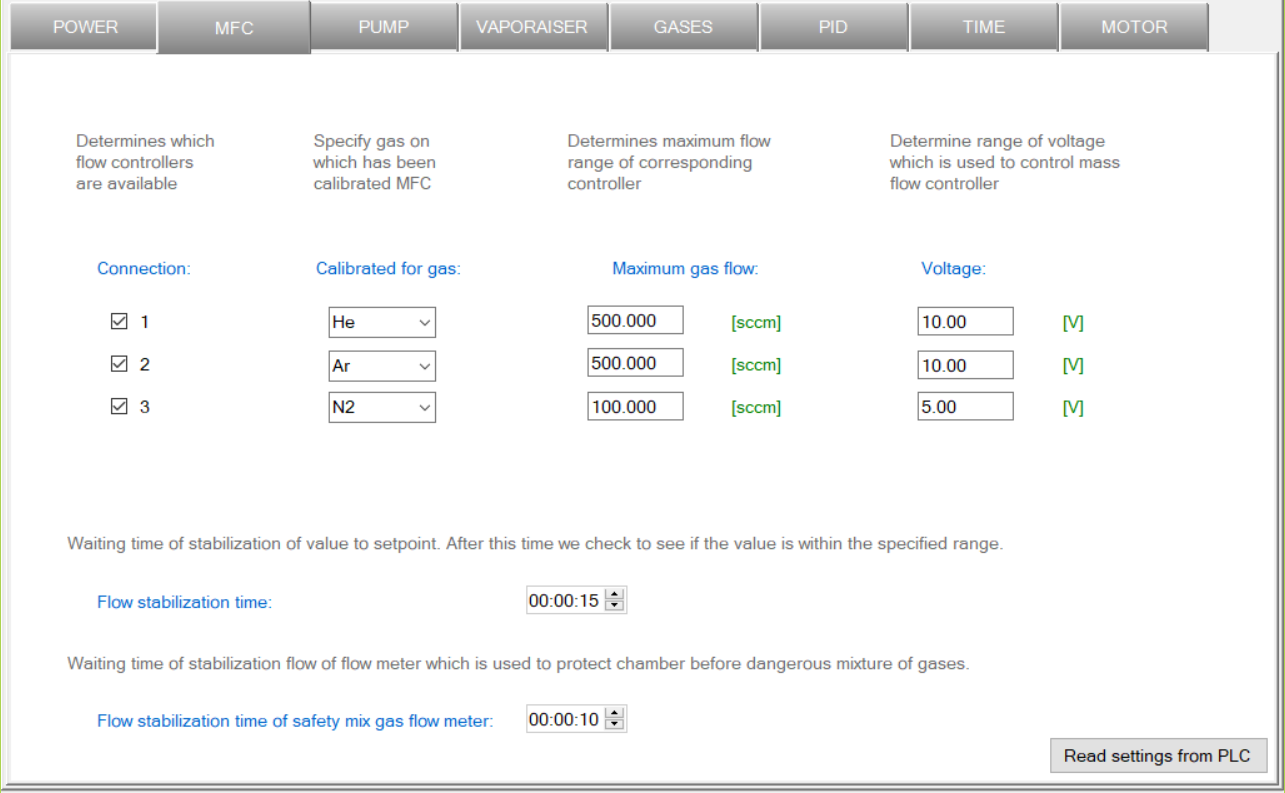
\includegraphics[width=0.8\textwidth]{Graphic/Service/MFC.png}	
	\caption{Service - section MFC}
	\label{alerts_window}
	\end{figure}
	\FloatBarrier

\subsection{Pump}

Section \textit{Pump} is used to configuration parameters of fore pump. We should specify time for wait of confirmation correctly turned on pump and time duration pumping down for line from pump to SV valve.\\\\
Parameters:
\begin{itemize}
\item \textit{Time wait on PF} - time for wait of confirmation correctly turned on pump. Confirmation is executed by check signal power from fore pump. When time passed and signal is in wrong state, pump reports error and we won't be able to pumping of chamber.
\item \textit{Time pump to SV} - time duration pumping down for line from pump to SV valve. In order to protect chamber before dirt, procedure pumping before open valve SV  pumped down his line.\\\\
Attention.\\
Too short time causes dirt on the chamber.
\end{itemize}

	\begin{figure}[!h] 
	\centering 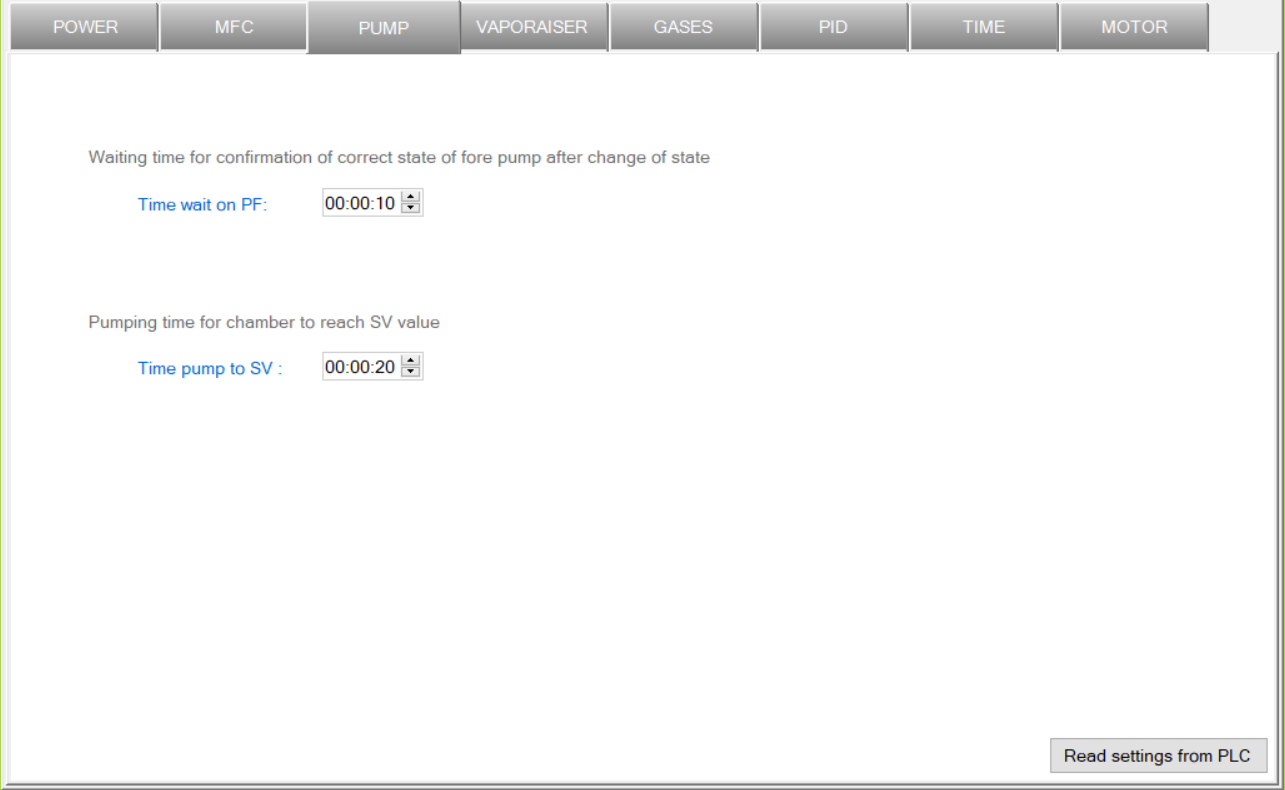
\includegraphics[width=0.8\textwidth]{Graphic/Service/Pump.png}	
	\caption{Service - section pump}
	\label{alerts_window}
	\end{figure}
	\FloatBarrier

\subsection{Vaporaiser}

Section \textit{Vaporaiser} specify what type of vaporaiser is used in system if system contains him. To determine type of vaporaiser we should select one of option from below: 
\begin{itemize}
\item \textit{None} - determine that system no contains vaporaiser 
\item \textit{Cyle} - determine that vaporiaser working as cycle of time. Gas is dosing by one of range time of cycle.
\item \textit{Dosing} - determine that vaporiaser working as injector gas. Gas is dosing by short shots injection of gas per minute
\end{itemize}
	\begin{figure}[!h] 
	\centering 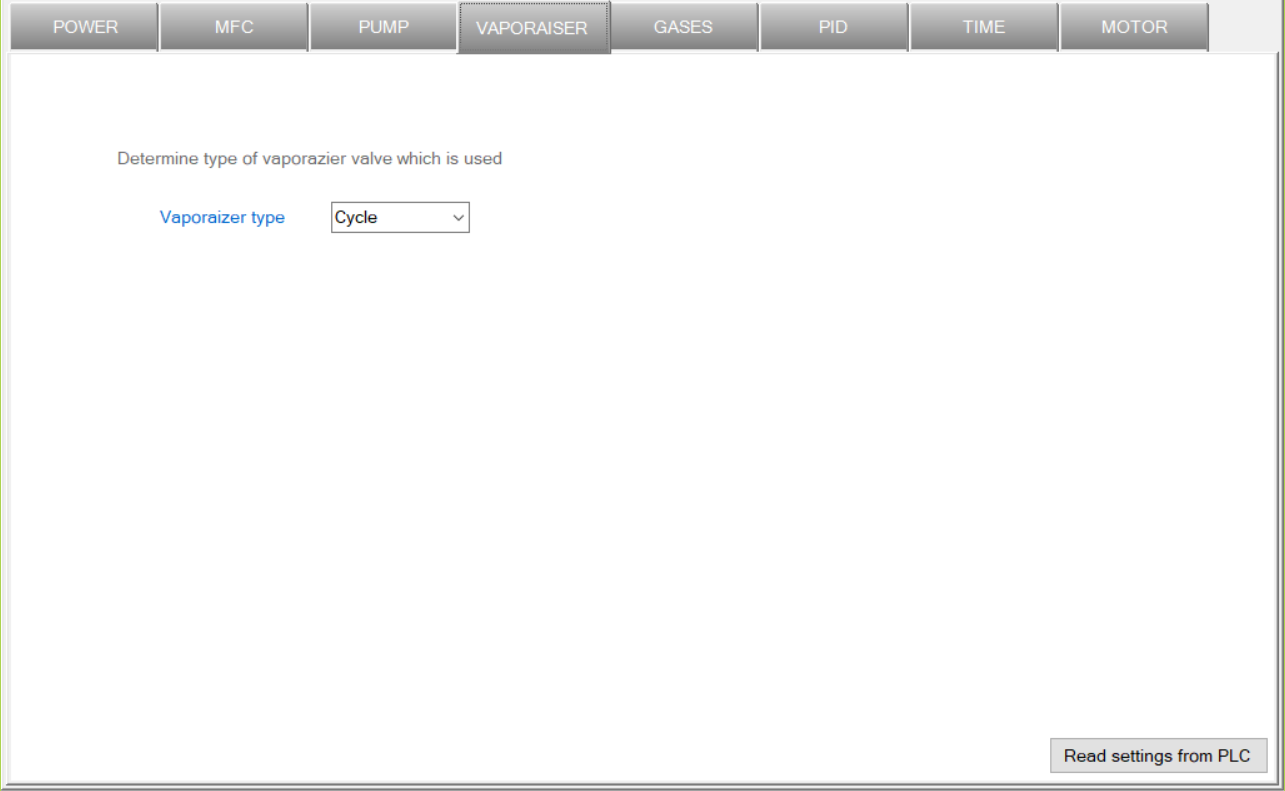
\includegraphics[width=0.8\textwidth]{Graphic/Service/Vaporaiser.png}	
	\caption{Service - section vaporaiser}
	\label{alerts_window}
	\end{figure}
	\FloatBarrier

\subsection{Gases}

Section \textit{Gases} allow us to determine list of gases which are used in system. We can also determine limit pressure for safe work of power supply and set limits of pressure for safe dosing gas to chamber.\\\\
Parameters:\\
\begin{itemize}
	\item  \textit{List gases} - displays all configured gases
	\item  \textit{Gas type in chamber} - determine correction of factor for measure gauge of pressure. 
	\item  \textit{Pressure limit for safe operation of power supply} - specify limit of pressure above which power supply will be emergency switched off
	\item  \textit{Pressure limit for gas injection} - specify limit of pressure above which dosing of gases to chamber will be emergency cut off
	\item  \textit{Flow limit to activate protect procedure} - specify limit of flow below which dosing of gases to chamber will be emergency cut off in order to protect chamber before dangerous mixture of gases. Flow is measuring on MFC3.
	\item  \textit{Enable protection} - enable/disable procedure protect before dangerous mixture of gases.
\end{itemize}

	\begin{figure}[!h] 
	\centering 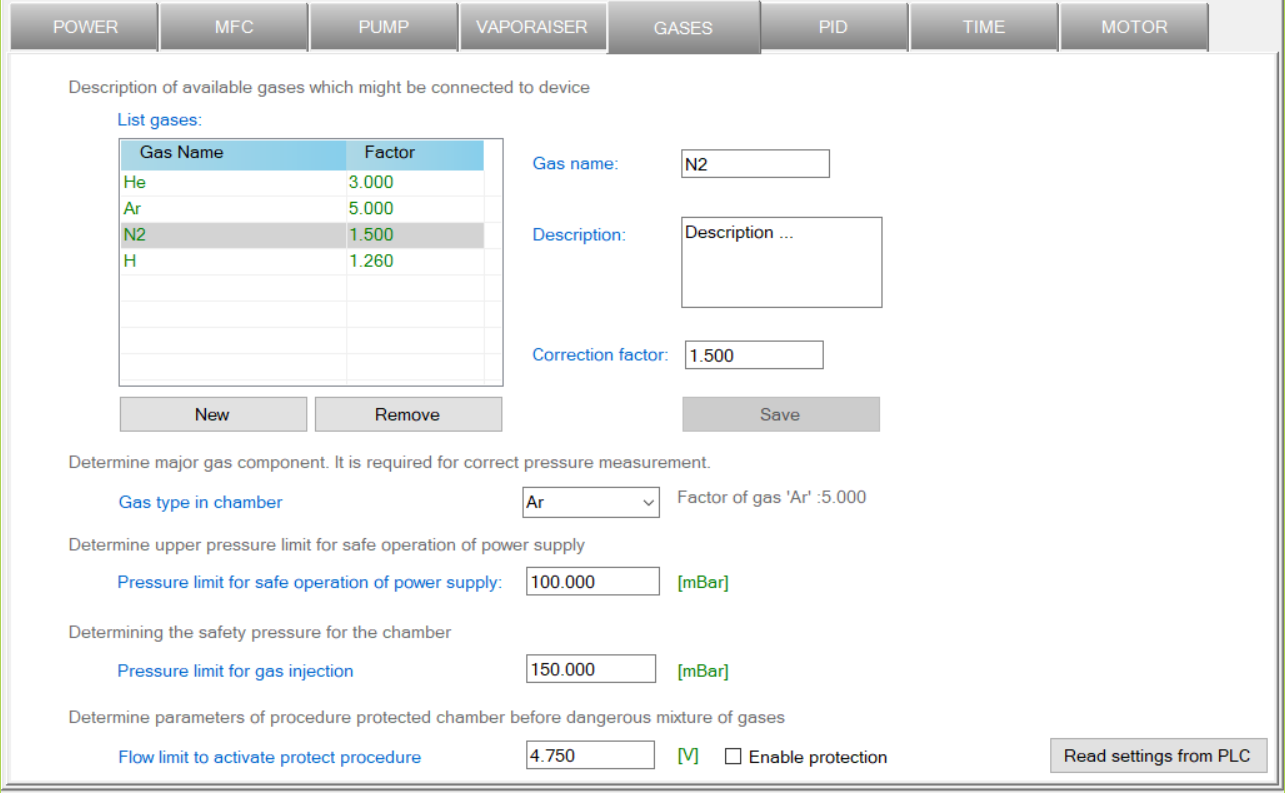
\includegraphics[width=0.8\textwidth]{Graphic/Service/Gases.png}	
	\caption{Service - section gases}
	\label{alerts_window}
	\end{figure}
	\FloatBarrier

\subsection{PID}

Section \textit{PID} allow us specify parameters of regulator PID. Regulator is used during automatically hold setting pressure in chamber.\\\\
Parameters:
\begin{itemize}
	\item \textit{Kp} - Proportional gain (0,01-100[times] => 1-10000[\%]). \\
	The proportional or gain term may be calibrated in two ways: Gain and Proportional Band.
	\begin{itemize}
	\item Gain = Output/Input. \\ 
			 Increasing the gain will cause the output to move more. 
	 \item Proportional Band is the \% change in the input which would result in a 100 \% change in the output.\\ 
	   	 Proportional Band = 100/Gain. 
	\end{itemize}
	\item \textit{Ti} - Integral time (0,1-3000[sec] => 1-30000[100ms], (>30000 = No integral effect)).\\ 
	The integral action is an action which continuously changes the manipulation value to eliminate a deviation when there is any. The time from the deviation occurence until the manipulation value of the integral action becomes that of the proportional control action is called the integral time and is indicated by Ti.\\
	The integral action is used in combination with the proportional action to form a PI action, or with the proportional and derivative actions to form a PID action.\\
	The integral action for the step response when the error value is constant is shown in the figure below.
	\item \textit{Td} - Differential time ( 0-300[sec] => 0-30000[10ms]; (0=>derivate function is disabled)).\\ 
	The derivative action adds the manipulation value proportional to the change speed to eliminate error when a deviation occurs.\\
	The time from the deviation occurence until the manipulation value of the derivative action becomes that of the proportional action is called the derivative time and is indicated by Td.\\
	The derivative action is used in combination with the proportional action as a PD action, or with the integrative action and the proportional action as a PID action.\\
	The derivative action for the step response when the deviation is constant is shown in the figure below.
	\item \textit{Ts} - Sampling cycle (0,01-60[sec] => 1-6000[10ms])
	\item \textit{Filtr} - Filter coefficient applied to the PV, 0-100[\%] => 0-100[\%]
	\item \textit{Pressure stabilization time} - determine wait time for stabilization of pressure. When time passed system will be check si pressure of chamber is in defined range by process.
\end{itemize}

	\begin{figure}[!h] 
	\centering 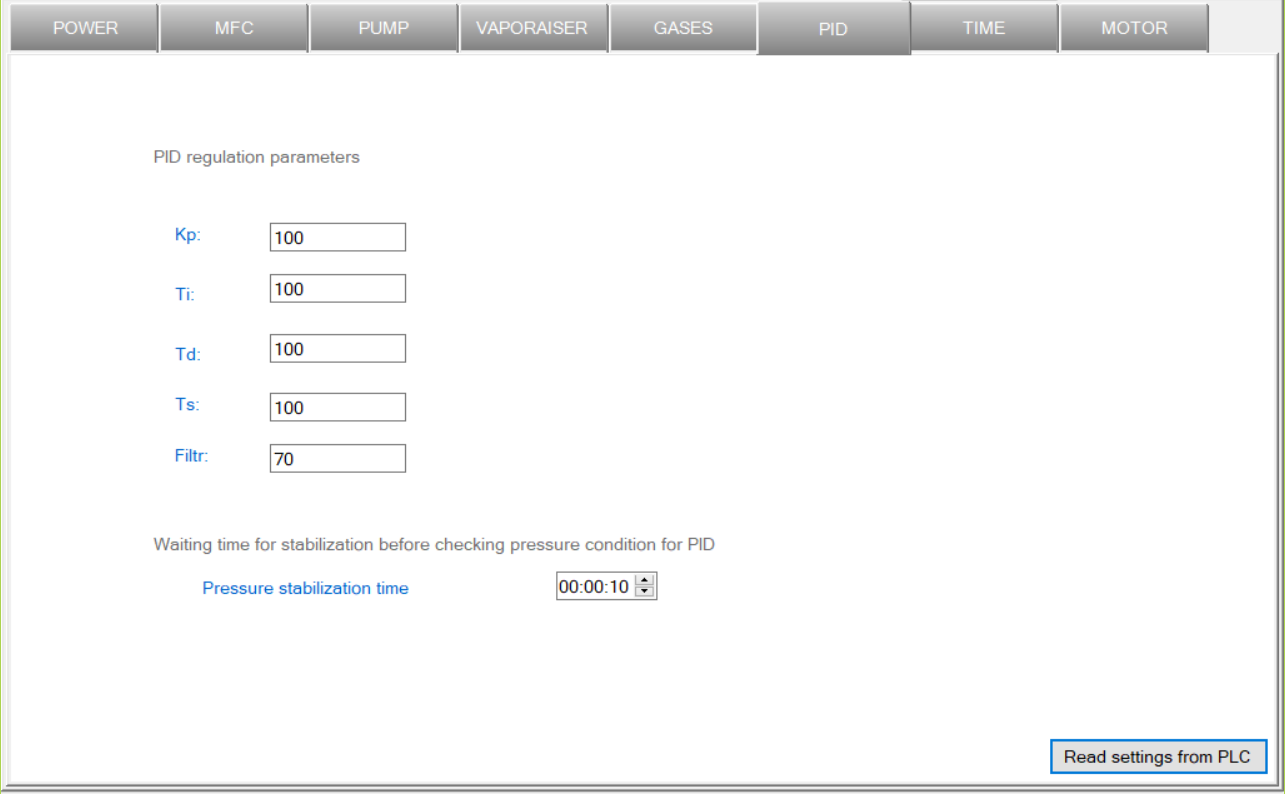
\includegraphics[width=0.8\textwidth]{Graphic/Service/PID.png}	
	\caption{Service - section PID}
	\label{alerts_window}
	\end{figure}
	\FloatBarrier

\subsection{Time}

Section \textit{Time} specify  time and date of controller machine (PLC driver).\\\\
Important.\\\\
Time of any errors is based for this setting

	\begin{figure}[!h] 
	\centering 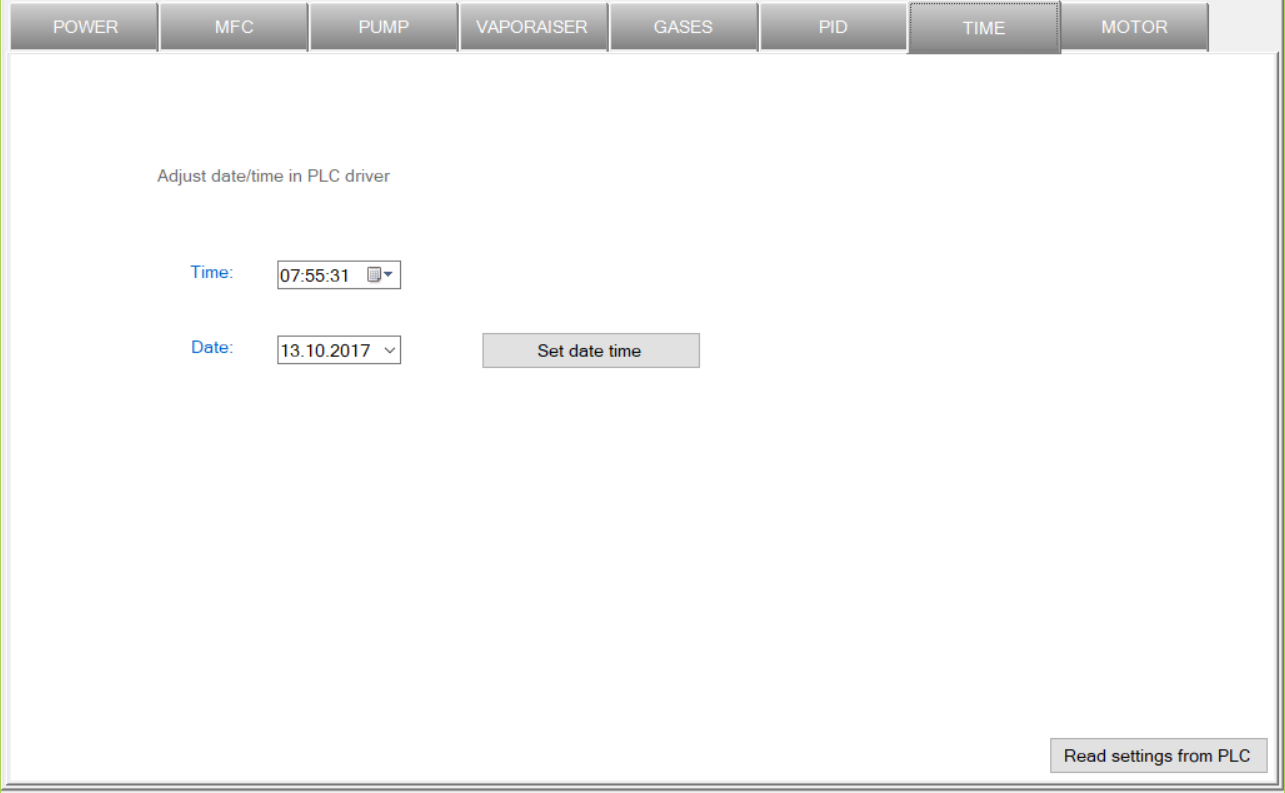
\includegraphics[width=0.8\textwidth]{Graphic/Service/Time.png}	
	\caption{Service - section time}
	\label{alerts_window}
	\end{figure}
	\FloatBarrier

\subsection{Motor}

Section \textit{Motor} define how many motors system contains

	\begin{figure}[!h] 
	\centering 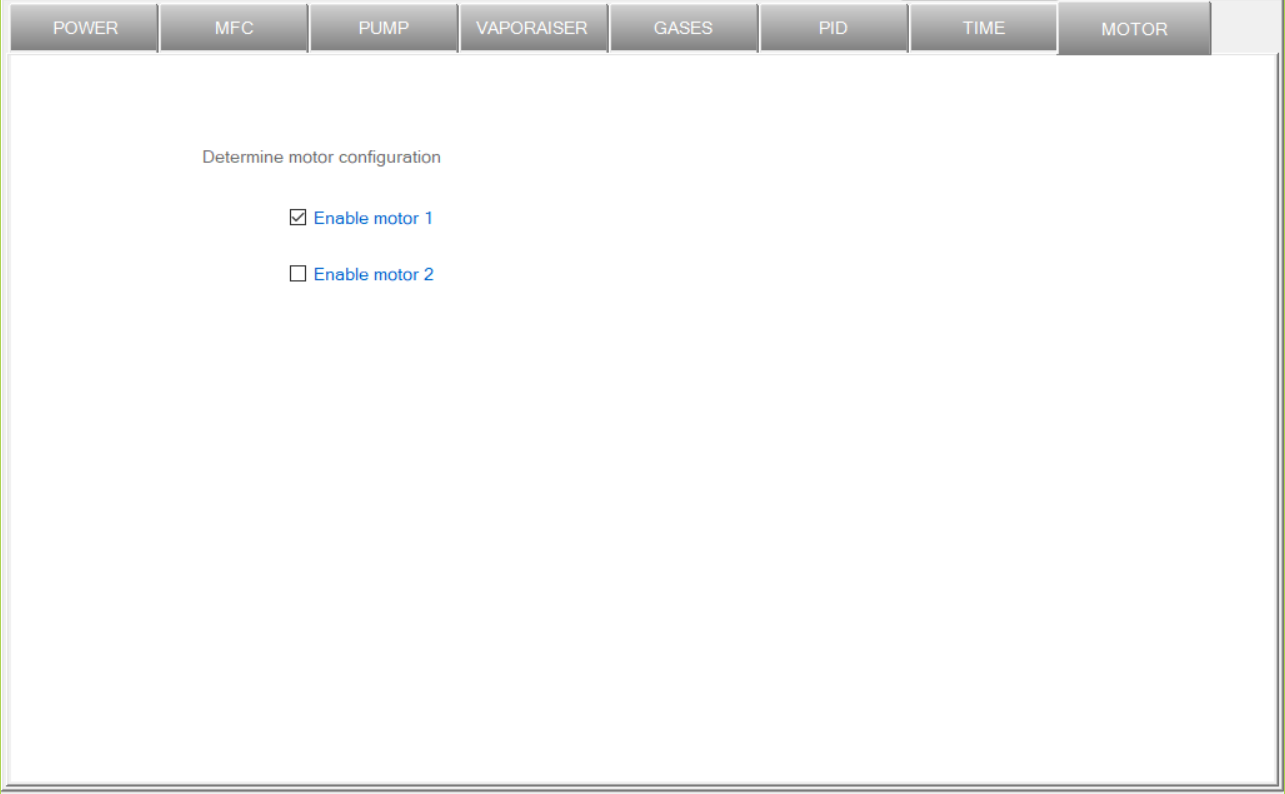
\includegraphics[width=0.8\textwidth]{Graphic/Service/Motor.png}	
	\caption{Service - section motor}
	\label{alerts_window}
	\end{figure}
	\FloatBarrier
